% -----------------------------------------------------------------------------
% Version 0.1
% -----------------------------------------------------------------------------

% \subsection{A Functional Approach to Pilot-Jobs}
% Many scientific communities began running into the same issues:

% As distributed systems grew in capacity and capability, they also grew
% in complexity and heterogeneity. For example, many machines
% implemented their own batch queuing systems, and oftentimes these
% systems varied from machine to machine.\msnote{The part after the
% comma is kind of implicit by the part before} The wide use of
% heterogenous resources, resulted in the need for workload management
% across these resources.  In order to harness the power of these
% heterogeneous resources to run jobs, one particular solution proposed
% is that of
% \pilotjobs

% , which have historically been used as a means of solving these
% issues. This gave rise to the the need for job submission management
% via batch queuing systems and middleware access also grew. We briefly
% discuss some specific uses of \pilotjobs below.

% \pilotjobs are most commonly used for the execution of many tasks
% through the use of a container job. They are often measured by their
% throughput, that is, the number of tasks that they can complete per
% second (tps)\msnote{I dont think we use tps further in the paper}, or
% alternatively, by the total number of tasks executed. As such,
% \pilotjobs are used to achieve high-throughput, for example, when
% using genome sequencing techniques \msnote{Arguably genome
% applications are not the most illustrative example of high throughput
% tasks getting benefit out of pilot-jobs} or ensemble-based
% applications. \pilotjobs have also been used for parameter sweeps,
% chained tasks, and loosely-coupled but distinct tasks. %note to self:
% cite these with papers

% Multi-scale simulations have also benefited from the use of
% \pilotjobs. A framework for load balancing via dynamic resource
% allocation for coupled multi-physics (MPI-based) simulations using
% \pilotjobs was demonstrated in Ref.~\cite{ko-efficient}. This was
% achieved by dynamically assigning more processors to jobs with longer
% runtimes, so that these jobs could accomplish their workload in the
% same amount of wall-clock time as those with shorter runtimes. This
% led to an overall reduction of jobs that were waiting to communicate
% via MPI, and an overall reduction of the total simulation runtime.

% \pilotjobs can be used for  simulations with varying numbers of tasks
%  to complete, for example, molecular dynamics simulations requiring
%  task restart. These types of simulations may start with a fixed
%  number of tasks but spawn more tasks in order to continue simulating.
%  \pilotjobs can be utilized for these types of dynamic simulations,
%  because new tasks can be fed to the \pilot at any time within a given
%  runtime. Without \pilotjobs, these simulations would have to be
%  resubmitted to the batch queue and wait for their time to become
%  active again~\cite{luckow2009adaptive}.

% \pilotjobs have also been used to avoid queue wait times for many jobs
% \msnote{I think we just said this above in the high-throughput case}
% as well as harness and utilize different resources (with different
% batch queueing systems) to do \textit{scale-across} simulations. As a
% fault tolerant mechanism, many \pilotjob systems monitor failed jobs
% and have the ability to restart them within the given time frame of
% the \pilotjob's total
% runtime~\cite{casajus2010dirac,frey2002condorG,nilsson2011atlas}.

% In order to appreciate \pilotjobs, we outline the evolution of
% \pilot-like capabilities ultimately leading to the creation of the
% first actual \pilotjob. We present a brief chronological order of
% \pilotjob-like systems, beginning with simple Master-Worker-based
% applications through advanced workload management systems.~\cite{}

% \subsubsection*{The Evolution of \pilotjobs}\label{sssec:evolution}

% \pilotjobs provide the ability to distribute workload across multiple
% systems and offer an easy way to schedule many jobs at one time. This
% in turn improves the utilization of resources\msnote{why?}, reduces
% the net wait time of a collection of tasks, and also prevents
% saturation of resource batch queuing systems from high-throughput
% simulations where many jobs need to be run at one time\msnote{I dont
% understand the last claim}. While early \pilot-systems solely provided
% this placeholder job mechanism, many of these system evolved to more
% complex workload management systems. As applications began to utilize
% distributed cyberinfrastructure, the workloads grew from small sets of
% short running jobs to many jobs with either short or potentially long
% runtimes. There was a need for more complex management of these
% workloads and additional capabilities for user-level control of the
% tasks that would be executed within the placeholder job. This drove
% the creation of the modern idea of \pilots \msnote{Kind of an ambigous
% statement, like all statements that include the word "modern" :-)}

% \pilotjob systems differ in their focus and architecture. Our
% preliminary survey of existing \pilotjobs helped to identify three
% major layers that these systems exhibit: (i) core \pilotjob
% functionality - this provides the minimally complete set of
% capabilities for a simple \pilotjob, (ii) advanced \pilotjob
% functionality - a system that offers all of (i) plus a more
% sophisticated resource management mechanism, and (iii) higher-level
% \pilot-based frameworks - frameworks utilize \pilots for a specific
% use case, e.\,g.\ workflows or data analytics.

% \onote{These are not necessarily 'layers'. The more I think about it,
% the whole idea of 'layers' doesn't make so much sense if we want to
% distinguish between core and advanced systems / frameworks. I think
% discussing these 'functionality' along \textbf{orthogonal components}
% (that doesn't necessarily build upon each other) would make more
% sense. My (and ALs) comment w.r.t Figure 1 is related to this.}
% \msnote{I'm tempted to at this stage in the paper use a very high
% level figure to simply support the explanation of the pilotjob
% concept.}

% As one can intuit from the above descriptions, existing \pilotjob
% systems maybe overlap and overflow into these different layers, and
% each layer builds upon the previous one. Therefore, we use these
% classification layers only as a means to explain the basic progression
% of a \pilotjob system from simple scheduling reservation mechanisms to
% more complete job management systems. A more semantically-rich
% terminology and classification scheme will be presented in Sections
% \ref{sec:vocab} and \ref{sec:analysis}.\msnote{I think the whole layering
% discussion can go.}


% Figure~\ref{fig:figures_classification} categorized \pilotjob systems
% into three layers: (i) core \pilotjob systems that solely provide a
% simple \pilot capability, (ii) advanced \pilotjob systems that offer
% sophisticated resource management capabilities based on \pilots, and
% (iii) higher level \pilot-based frameworks that utilize \pilots for a
% specific use case, e.\,g.\ workflows or data analytics. One of the
% important aspects of these layers is that they often overlap or have
% evolved from one another. Therefore, it is hard to classify

% \begin{figure}[t]
%   \centering
%       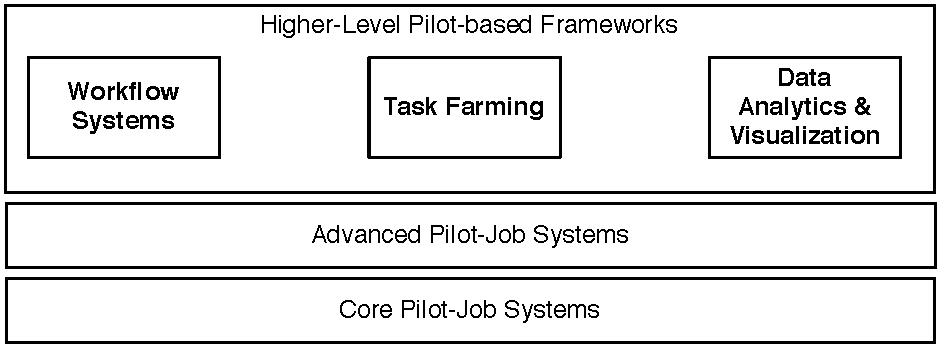
\includegraphics[width=0.45\textwidth]{figures/classification}
%   \caption{Pilot-Job Classification: Different PJ systems focus
%         on different parts of the distributed computing stack: (i)
%          PJ systems that solely provide the \pilot capability, (ii)
%          systems that offer resource management capabilities based on
%          \pilots and (iii) applications, tools and services that
%          utilize \pilots for resource management. \jhanote{we should
%            make the three levels of the diagram consistent with the
%            three categories, ``core PJ'' , ``advanced PJ'' and
%            ``higher-level PJs'' . Also earlier comment about adding
%            ``higher-level pilot-based frameworks'' to ``higher-level
%            frameworks that can use pilot-jobs''.}}  \alnote{mention
%          that these layers are not cleanly separated, add
%          capabilities (outside)/properties (internal) of
%          each layer, what is the overlap between the layers (how they
%          interrelated?, what is the overlap?)?}
%          \onote{IMHO this figure doesn't really help to explain things
%          and is also wrong (see AL's comment above). I think we should
%          get rid of it.  } \msnote{+1}
%   \label{fig:figures_classification}
%\end{figure}

% In this section, we give a brief overview of different \pilotjob
% systems. As grid computing advanced in its size and capabilities, the
% need for job scheduling and time-sharing became more prevalent. Batch
% queuing systems were installed to solve this problem, wherein a login
% node accepted all job submissions and then the queuing system divided
% the work to the worker nodes. The requirements of distributed
% applications, such as efficient load balancing and resource
% utilization across multiple resources, drove the need for user-level
% control of tasks and ease of use of job descriptions for data driven
% applications~\cite{ko-efficient}~\cite{DBLP:conf/hpdc/KimHMAJ10}, but
% the concept of a \pilot was not the first type of application-level
% scheduling introduced.

% -----------------------------------------------------------------------------
% Version 0.2
% -----------------------------------------------------------------------------

% , it was an early mentioning of large scale parallel computing. In
% determining the necessary processing power for weather forecasting, he
% estimated that 64000 human \textit{computers} would be required for solving
% the equations. These computers would all be assigned a part of the globe by a
% central \textit{senior clerk}. The computers would perform their calculations
% and the results would be collected by the clerk. This was in effect a
% Master-Worker pattern.

% \jhanote{Mark: I propose the following: One common use for the M-W scheme is
% to serve as the coordination substrate for PJs. I know its a bit nebulous,
% but it connects the two concepts directly, which is the goal here.}
% \msnote{Interesting contrast. Do we see M/W as a communication pattern to
% implement PJs or do PJs enable the M/W pattern to applicatons?}
% \mtnote{Please see~\S\ref{sec:compsandfuncs}, 10th paragraph: "As see in..."}

% As established in the introduction, \pilotjobs have proven to be an effective
% tool for task-level parallelism. \mtnote{Do we introduce task-level
% parallelism explicitly?} (Note that the current term \textit{\pilotjob} is not
% as old as the concept itself, and the word \pilot for this concept was likely
% introduced around 2004 in the context of the LHC data challenge.
% \alnote{the concept or the name? figure 2 goes back way further than 2004}
% It's first written appearance is in a 2005 LHCb report\cite{nobrega2005lhcb}).
% \msnote{find a nice place for this line} One common use for the \pilotjob
% paradigm is to enable the Master-Worker (M-W) scheme \mtnote{We use pattern
% istead of schema in the next paragraph.} and its associated frameworks for
% applications~\cite{Shao:2000:masterslave}.

% When Lewis Fry Richardson in 1922 devised his \textit{Forecast Factory}
% (Figure~\ref{fig:figures_forecast-factory}), it was an early mentioning of
% large scale parallel computing. In determining the necessary processing power
% for weather forecasting, he estimated that 64000 human \textit{computers}
% would be required for solving the equations. These computers would all be
% assigned a part of the globe by a central \textit{senior clerk}. The computers
% would perform their calculations and the results would be collected by the
% clerk. This was in effect a Master-Worker pattern.

% Figure~\ref{fig:timeline} shows the introduction of the discussed systems and
% terms. When available, the date of first mention in a publication or otherwise
% the release date of software implementation is used.

% In the context of present distributed systems, the M-W scheme was initially
% used for farming tasks from a master to a various number of workers, and could
% easily be adapted to run in a platform-independent way across potentially
% heterogeneous resources~\cite{masterworker, Goux00anenabling}. M-W based
% frameworks could respond to dynamically changing resources by adapting the
% number of workers to match the resource availability.\mtnote{Should this
% paragraph be expanded so to include some description/example of the referenced
% distributed systems and capabilities?}

% As distributed computing infrastructures became more popular and available,
% user demand drove the need for efficient shared allocation of heterogeneous
% resources. Leveraging the batch processing concept, first used in the time of
% punchcards [ref], job schedulers were created to accommodate these needs,
% often called ``batch queuing systems''. The adoption of batch queuing meant
% users were expected to submit their tasks to the job scheduler (queue) of each
% cluster and grid system.
% \msnote{From here its an obvious (side)-step to meta scheduling?}

% Often, the type of scheduler on a one machine was different than that of
% another machine. Clearly, there was a need for managing these heterogeneous,
% dynamic grid environments, especially in terms of dynamic scheduling.

% \ldots

% This pattern was implemented with manageable overheads and could easily be
% adapted to run in a platform-independent way across potentially heterogeneous
% resources~\cite{masterworker, Goux00anenabling}. M-W based frameworks could
% respond to dynamically changing resources by adapting the number of workers to
% match the resource availability.\mtnote{To be aggregated in the new version}

% \ldots

% \msnote{\cite{Gehring:1996:mars} looks just as relevant and predates apples:
% "... Note: AppLeS more active than MARS now MARS uses accumulated statistical
% data on previous execution runs of the same application to derive an improved
% task-to-process mapping"}.

% Commented out GHS for now.
%
% The rise of application-level scheduling, as in AppLeS, opened new
% possibilities to Grid environments. The concept of application-level
% scheduling was extended to include long-term performance prediction in
% heterogeneous Grid environments via the Grid Harvest Service (GHS)
% system~\cite{ghs}. GHS provides a prediction model that was derived by
% probability analysis and simulation and useful for large-scale applications
% in shared environments. Its prediction models and task scheduling algorithms
% are utilized in the placement of tasks across Grid resources. GHS supports
% three classes of task scheduling: (i) single task, (ii) parallel processing,
% and (iii) meta-task. The performance evaluation and modeling in conjunction
% with task-specific management (such as placement, scheduling, and execution)
% allows the utilization of many heterogeneous resources in an efficient manner.

% complexities of task management and coordination to the application layer.
% In order to isolate the application itself from the scheduling of resource
% placeholders,

% , due to its design it required changes to the application itself. For
% obvious reasons this is not always a desired situation and there was a need
% to have user-level control of scheduling without altering the original
% application. This brought about the idea of placeholder scheduling.


%  in that it was an abstraction layer above the various batch
% queuing systems available on different resources. It held a \textit{place} in
% the regular batch queue, and when it became active, it could pull tasks to
% execute.

%Core \pilotjob systems focus on the basic \pilot capabilities, i.\,e.\ the
%provisioning of the placeholder job capability. Various Master-Worker systems
%that provide such a mechanism (e.\,g.\
%Nimrod-G~\cite{buyya2000nimrod}). Condor-G/Glide-In is the most
%well-known \pilotjob system.  \msnote{Im tempted to not make claims like this,
%especially not without backing up.}

%Further examples for lightweight \pilotjob systems are: ToPoS~\cite{topos},
%MyCluster~\cite{Walker:2007:PAC:1285840.1285848}, MySGE~\cite{mysge},
%GridBot~\cite{Silberstein:2009:GEB:1654059.1654071} and LGI~\cite{lgi}.

%Nimrod-G~\cite{buyya2000nimrod}, DIANE~\cite{diane-thesis} and Work
%Queue~\cite{workqueue-pyhpc2011} are examples of Master-Worker systems that
%utilize a placeholder agent that dispatches and manages tasks. For example,
%Nimrod-G utilizes a Job Wrapper that is responsible for pulling a task and its
%associated data and then manages the execution of this task. While modern
%\pilotjobs often acquire resources opportunistically and then distribute tasks
%to resources they were able to acquire, Nimrod-G utilizes a central,
%cost-based scheduler.\msnote{Is this really a distinction, arent most of the
%systems centrally controlled?}

% Applications can be built on top of BOINC for their own scientific endeavors.
% \mrnote{As just an end reader, it is really unclear how this relates to
% anything. Is this supposed to follow from the previous para?}
% \aznote{Yes -- perhaps combine this + last para?  maybe even next para
% too...}

% A Glide-in is submitted using the Condor-G grid universe \msnote{Is this a
% distinctive feature? Arent the universes just labels anyway?}. On the remote
% resource a set of Condor daemons is started, which then registers the
% available job slots with the central Condor pool. The resources added are
% available only for the user who added the resource to the pool, thus giving
% complete control over the resources for managing jobs without any queue
% waiting time. Glide-in installs and executes necessary Condor daemons and
% configuration on the remote resource, such that the resource reports to and
% joins the local Condor pool. Various systems that built on the \pilot
% capabilities of Condor-G/GlideIn have been developed, e.\,g.\

% Glide-in is limited in that the daemons must be running on a given resource,
% meaning that this process must be approved by resource owners or system
% administrators.

% Venus-C~\cite{venusc-generic-worker} provides a \pilotjob-like capability on
% Microsoft Azure clouds called a Generic Worker. The Generic Worker creates a
% layer of abstraction above the inner workings of the cloud.  The idea behind
% the Generic Worker is to allow scientists to do their science without
% requiring knowledge of backend HPC systems by offering e-Science as a
% service. Venus-C has not been shown to work with grids, because its main
% objective is to motivate scientists to use cloud infrastructures.  While the
% notion of moving to the cloud for data-driven science is an important one,
% many existing cyberinfrastructures still have powerful grid computers that
% can also be leveraged to assist with the data-driven computations.

% In addition to the \pilotjob systems developed around the LHC experiment,
% several other systems emerged. Commented out gwpilot. Not really
% published/downloadable, and no obvious new functionality.
% GWPilot~\cite{gwpilot} is a \pilot system that is developed as a component
% for the GridWay meta-scheduler. GWPilot emphasizes its easy deployment,
% multi-user support and the support of standards, such as DRMAA, OGSA-BES and
% JSDL.
% \jhanote{will need references to these obscure acronyms!}
% \jhanote{Furthermore, must check that the reference to GWPilot is kosher. No
% bacon allowed.}
% \mrnote{It seems a little awkward that we say several others have emerged,
% then we say gwpilot is one. but then we go into talking in next para about
% scientific workflows + pjs. Several makes it sound like we have a bunch more
% to discuss}
% \msnote{In what way are these systems intrinsically pilot based? I think for
% example with Pegasus, it can make use of pilots, but uses it as just yet
% another "job submission backend". In this way, any system that creates "task"
% could be adopted to submit to a pilot-based backend}

% Many higher-level tools and frameworks, such as workflow, visualization or
% data analytics systems, utilize \pilotjob systems to manage their
% computational workload. In general, two approaches exist: (i) the framework
% vertically integrates with a custom \pilotjob implementation (e.\,g.\
% Swift/Coaster) or (ii) it re-uses a general purpose PJ system (e.\,g\
% Pegasus/Condor-G). In case (i), the PJ system is also often exposed as
% stand-alone, multi-purpose \pilotjob systems.

% In contrast to GlideinWMS, Corral-Glide-Ins are run using the credential of
% the user and not a VO credential. Workflow task clustering with
% Pegasus~\cite{Singh:2008:WTC:1341811.1341822}.

% For this purpose, Swift formalizes the way that applications can define
% data-dependencies. Using so called mappers, these dependencies can be easily
% extended to files or groups of files. The runtime environment handles the
% allocation of resources and the spawning of the compute tasks. Both data- and
% execution management capabilities are provided via abstract interfaces.

% Using the Coaster service, one executes a Coaster Master on a head node, and
% the Coaster workers run on compute nodes to execute jobs. In the case of
% cloud computing, Coasters offers a zero-install feature in which it deploys
% itself and installs itself from the head node and onto the virtual machines
% without needing any prior installation on the machine.
% \msnote{Where does the virtual machine suddenly come from?} Coaster relies on
% a master/worker coordination model. communication is implemented using
% GSI-secured TCP sockets. Swift supports various scheduling mechanisms on top
% of Coaster, e.\,g.\ a FIFO and a load-aware scheduler.
% \jhanote{I think the previous paragraph can be highly reduced. The next
% paragraph should be modified to highlight that {\bf specialized} pilots have
% also emerged, namely falkon to support many short running jobs on HPC
% systems. This is an important point to make and speaks to the success of the
% pilot concept}

% Falkon refers to pilots as the so called provisioner, which are created using
% the Globus GRAM service. The provisioner spawns a set of executor processes
% on the allocated resources, which are then responsible for managing the
% execution of task. Tasks are submitted via a so called dispatcher service.
% Falkon also utilizes a master-work coordination model, i.\,e.\ the executors
% periodically query the dispatcher for new tasks.

% Web services are used for communication\msnote{between?}.

% WISDOM~\cite{Ahn:2008:ITR:1444448.1445115,wisdom} is an application-centric
% environment for supporting drug discovery. The architecture utilizes an agent
% run as a Grid job to pull tasks from a central metadata service referred to
% as AMGA.
% \jhanote{this paragraph/pilot can go. I don't see the new functional feature
% or increased complexiy that WISDOM introduces}

% A LRMS incorporating a pilot scheme:
% OAR~\cite{oar} is a batch scheduler system for clusters and other
% computing infrastructures. Besides its more traditional batch scheduler
% features, it also has the functionality of \textit{container jobs}. These type
% of jobs allow the execution of jobs within other jobs, effectively making it a
% sub-scheduling mechanism, and thereby making it a batch scheduler with
% \pilotjob capabilities.

% Maybe add netsolve later:
% NetSolve~\cite{Casanova:1995:NNS:898848}

% -----------------------------------------------------------------------------
% Version 0.3
% -----------------------------------------------------------------------------
